\chapter{Learning Room Occupancy Based On User Routines}
\label{chapter:occupancy}
In this chapter, we investigate how a robot can learn occupancy period of different rooms of an office or home based on users' routine. Occupancy represents the belief of the robot about whether a particular room will be occupied or empty. 

We consider the example of a cleaning robot which needs to decide what time of the day is best suited for cleaning of a specific room. \cite{Fink2013},  did an exhaustive survey about usage, adoption process and long-term effects of domestic cleaning robot in people's homes. \citeauthor{Fink2013} observes that one of the biggest barriers for better adoption of robots in households was compatibility with habits and routines. Thus, in order for a robot to clean a house or office with minimum intervention, the robot should have the ability to understand its user's routines. One of the aspects the robot can learn about the user's routine will be what time the user prefers to use each room. From the robots perspective, it would be to learn the occupancy of each room. Based on the occupancy of each room, the robot can plan to clean the room during time periods of minimum occupancy, thus causing minimum interference for the users.

In this chapter the robot will learn multiple users' routine in using different rooms of a office and determine the low occupancy time for cleaning.
The robot is assumed to use internal sensors and standard person detection algorithm to detect the human \cite{linder16multi, jafari2014real}. This generated information is recorded by the robot in its robot memory along with the time and room of the observations. We explain a probabilistic model which can learn from these observations and generate the occupancy periods for each room. In particular, our approach allows a robot (1) to infer the occupancy of each room from previous observations (2) to make predictions about future occupancy of each room. In our experiments, we demonstrate that robots with our models can learn and predict accurately if a room is occupied.


  \begin{minipage}{\textwidth}
  \begin{minipage}[b]{0.49\textwidth}
    \centering
        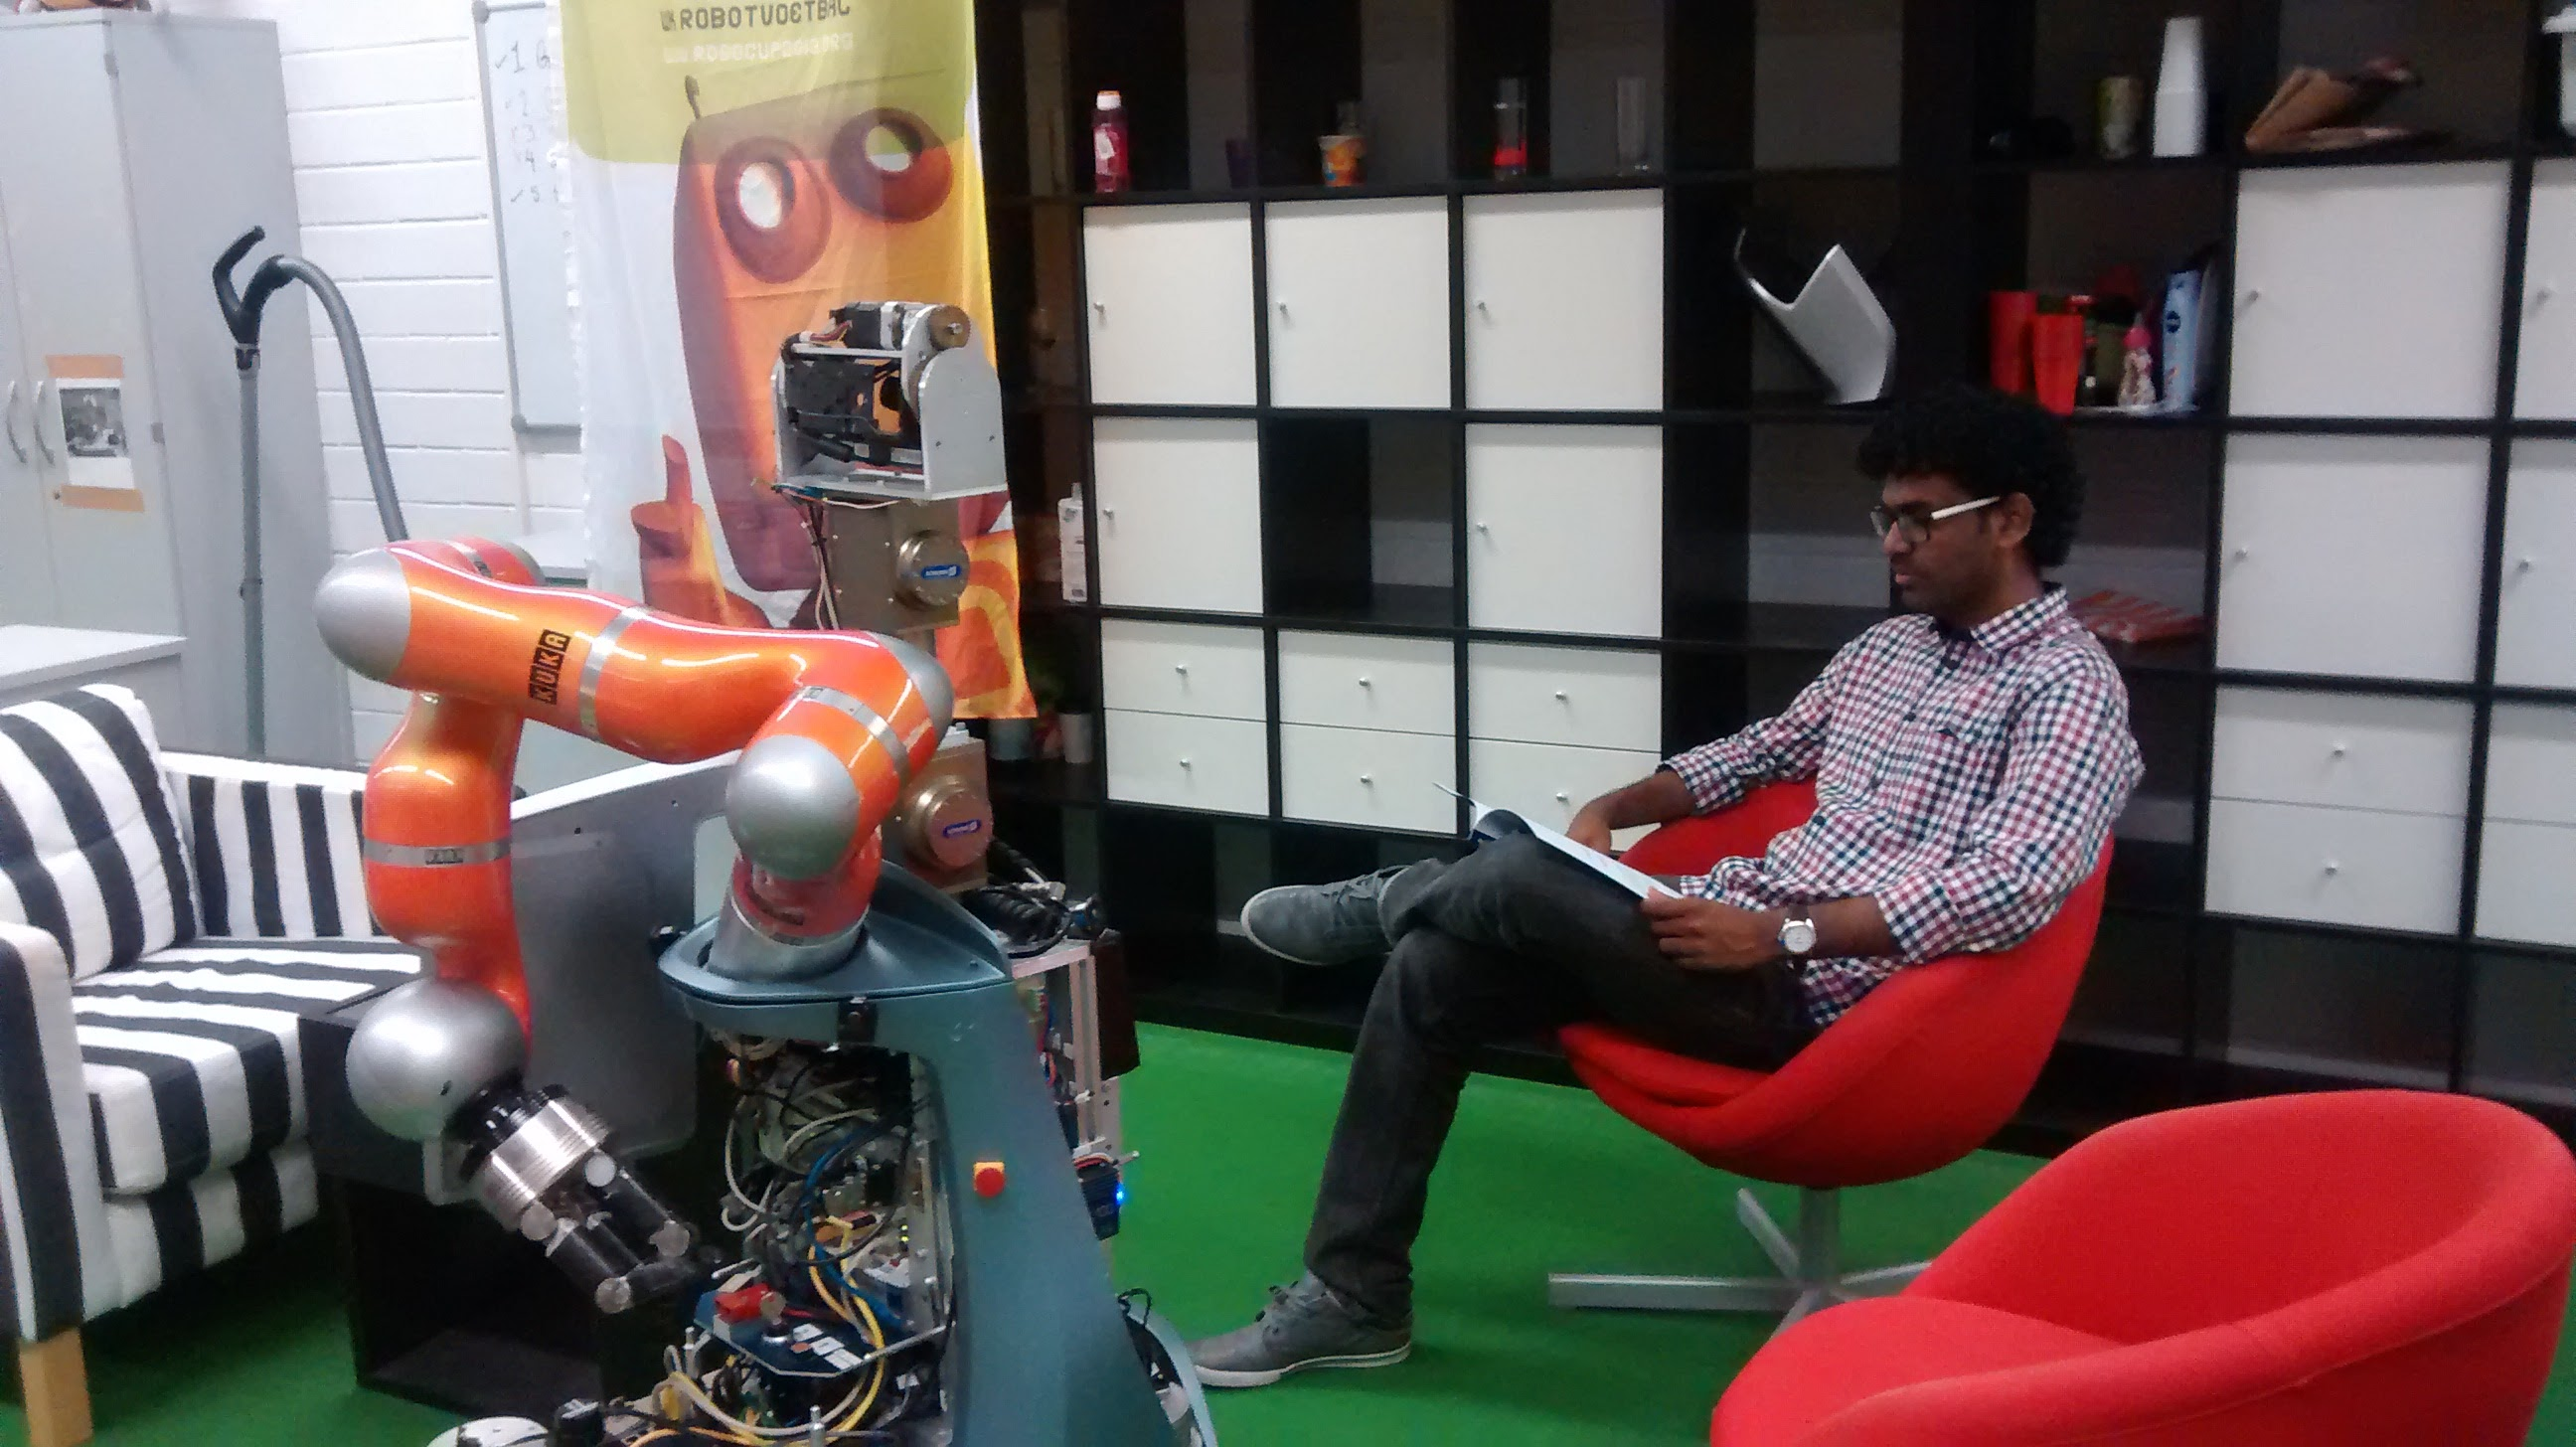
\includegraphics[width=0.9\textwidth]{images/cleaning_1.jpg}
    \captionof{figure}{Robot scanning living room}
    \label{fig:user_scan}
  \end{minipage}
  \hfill
  \begin{minipage}[b]{0.49\textwidth}
    \centering
    \begin{tabular}{|l|l|l|}
        \hline
	        Time & Location &  Occupied\\
        \hline
        \hline
	        09.03 & living room & True\\
        \hline
	        09.13 & living room & True\\
        \hline
	        09.23 & kitchen &  True\\
        \hline
	        09.45 & bedroom &  True\\
        \hline
	        09.53 & bedroom &  False\\
        \hline
	        10.03 & kitchen &  False\\
        \hline
        \end{tabular}
      \captionof{table}{Robot memory}
      \label{tab:robot_memory}
    \end{minipage}
  \end{minipage}


\section{Approach}

We formulate the problem of occupancy by modelling the belief of finding any person in the particular room at that time. Robot whenever scans a particular room as illustrated in Figure~\ref{fig:user_scan}, it records in its memory if the room was occupied or vacant. Thus the observations made by the robot are boolean variable, True for occupied and False for vacant. For modelling this boolean observation over multiple time periods we use the Hierarchical Beta Bernoulli model.


\section{Hierarchical Beta Bernoulli Model}

The Hierarchical Beta Bernoulli model explained in Chapter~\ref{chapter: object} is also used to model the occupancy of each room. In Chapter~\ref{chapter: object} the observations were boolean value representing the presence of an object at a particular location while the observations here is a boolean value representing if the room is occupied. From these boolean observations we need to learn the latent knowledge about occupancy. Bernoulli distribution is used to represent the observations, while the latent occupancy of the room is represented by the Beta distribution. 
Now the model learns the latent knowledge about the occupancy separately for each hour of the day. To enable sharing of knowledge between different times of the day we use the third level of the model.
\noindent
\begin{figure}[htp]


\begin{minipage}{0.3\textwidth}
\centering

\tikz {
 % Define nodes
  \node[latent]                                 (theta) {$\theta$};
  \node[latent, above=of theta, xshift=-1.2cm]  (alpha) {$\alpha$};
  \node[latent, above=of theta, xshift=1.2cm]   (beta) {$\beta$};
  \node[obs, below=of theta]                    (y)     {$x$}; 
  % Connect the nodes
  \edge {alpha,beta} {theta} ; %
  \edge {theta} {y};
  % plates
  \plate {location} {(y)} {location};
  \plate {time} {(theta)(y)(location)} {time};
}

\end{minipage}%
\begin{minipage}{0.7\textwidth}

\begin{equation*}
	\alpha \sim Beta(2,2) ; \beta \sim Beta(2, 2);
\end{equation*}
\begin{equation*}
	\theta \sim Beta(\alpha, \beta);
\end{equation*}
\begin{equation*}
	x = Bernoulli(\theta)
\end{equation*}
\end{minipage}
\caption[Hierarchical Beta Bernoulli graphical model]{Graphical model representation of Hierarchical Beta Bernoulli model. The boxes are ``plates" representing replicates. The outer plates represents hours of a day, while the inner plate represents if the room has users in that hour.}
\label{bbm2}
\end{figure}



The model can be explained as:

	\boldmath{$\alpha$} and \boldmath{$\beta$} is  prior beta distribution, 
	
	$\theta_i$ is the latent occupancy for period $i$  ,
	
	$x_{ij}$ is the human presence observation in period $i$.



\FloatBarrier
\section{Experiments}
We conducted our experiments on real data collected by a robot in an office environment. The robot for each room in the office makes an observation regarding it's occupancy. The goal of the experiment is to verify that
\begin{itemize}
    \item the robot is able to learn the room occupancy probability.
	\item the resulting model allows for accurate prediction or future occupancy of the room
\end{itemize}


\begin{figure}
    \centering
    \begin{subfigure}[b]{0.21\textwidth}
        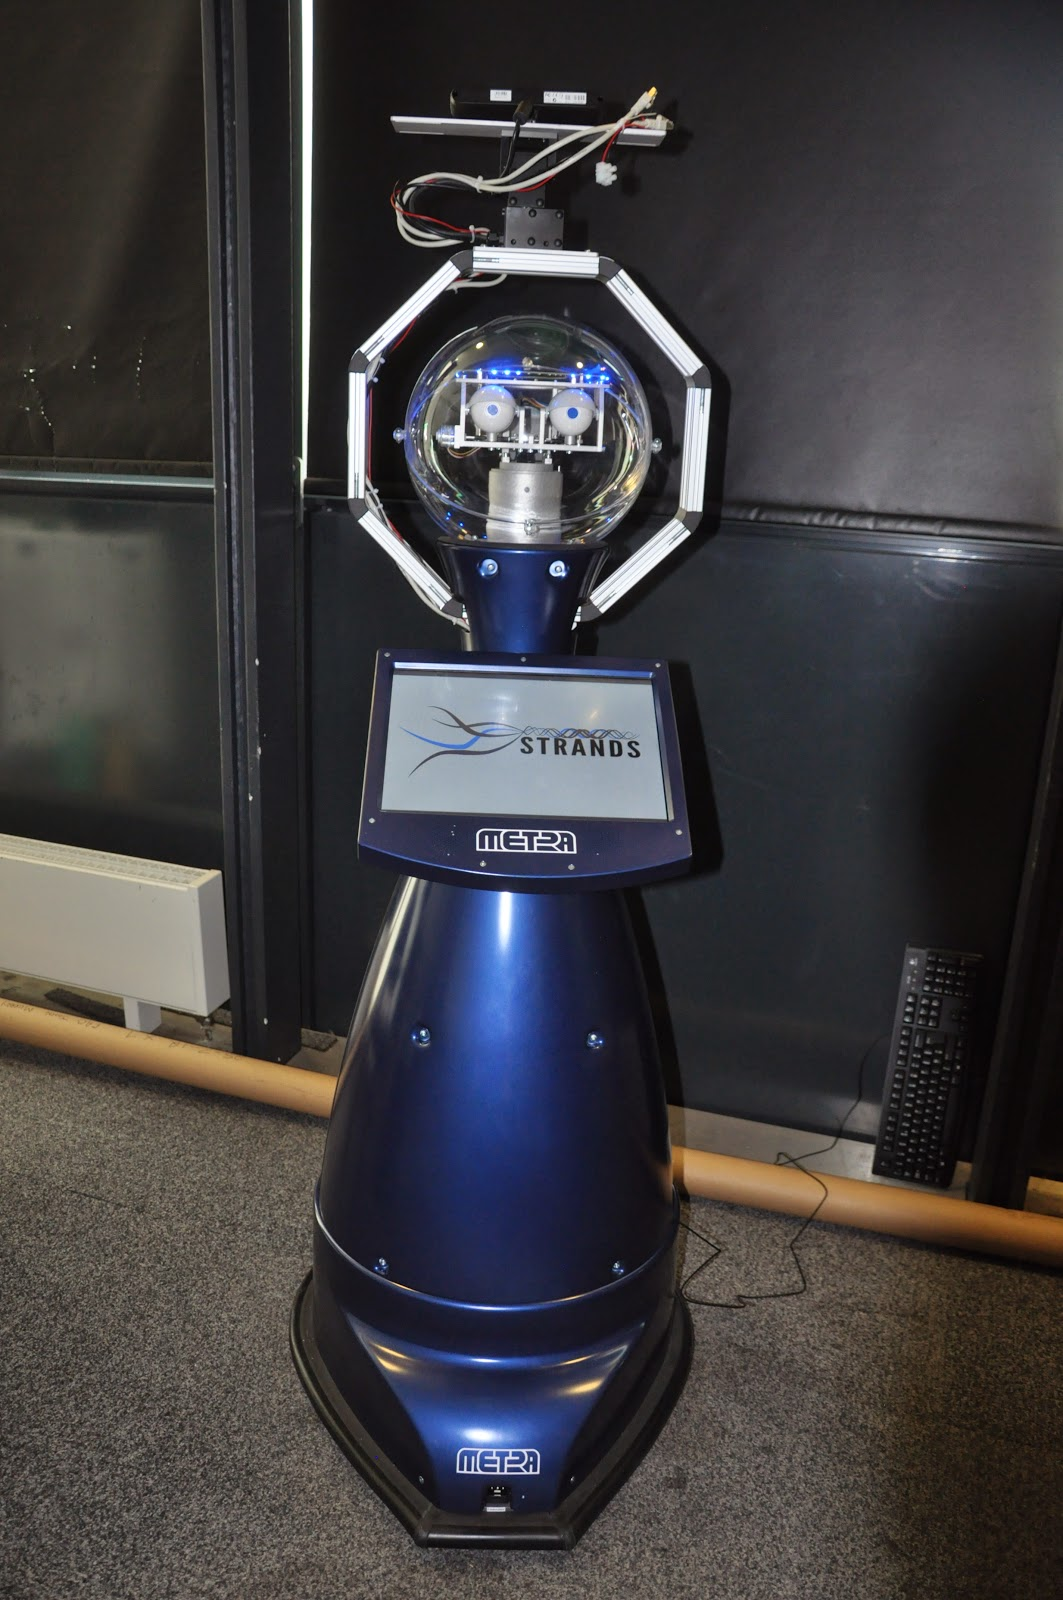
\includegraphics[width=\textwidth]{images/scitos.jpg}
        \caption{}
        \label{fig:scitos}
    \end{subfigure}
    ~ %add desired spacing between images, e. g. ~, \quad, \qquad, \hfill etc. 
      %(or a blank line to force the subfigure onto a new line)
    \begin{subfigure}[b]{0.6\textwidth}
        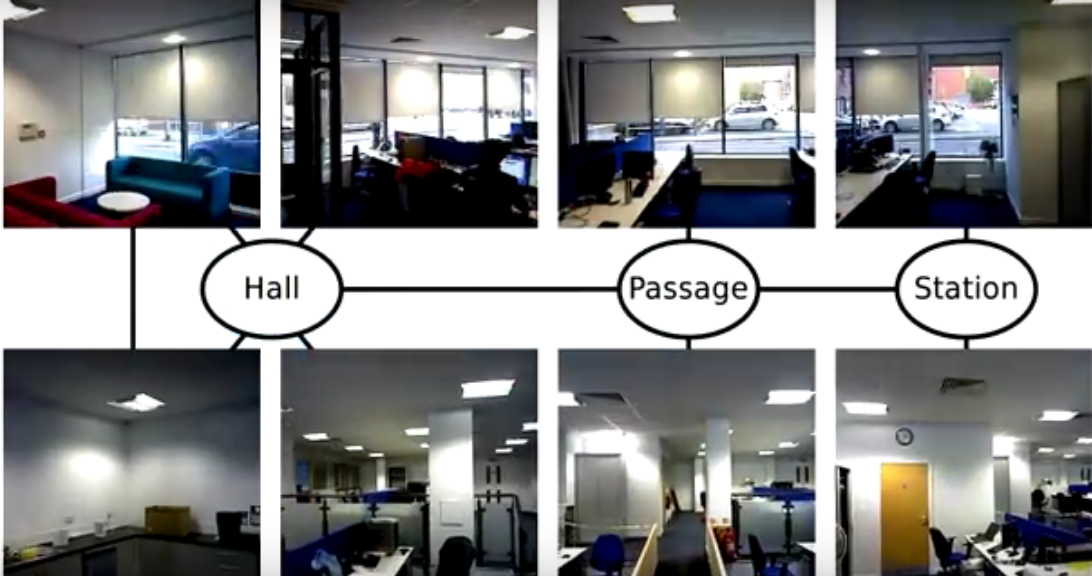
\includegraphics[width=\textwidth]{images/kth-dataset-2.png}
        \caption{}
        \label{fig:robot-view}
    \end{subfigure}
    \caption[Brayford dataset collection]{Brayford Dataset collection: \cite{SCITOS_G5} Robot used for data collection. Images  as seen by the robot at the different waypoints in the lab \citep{krajnik_wheres_2015} }\label{fig:brayford-dataset}
\end{figure}

\FloatBarrier
\subsection{Evaluation Of Model Accuracy}

We evaluated the model on the Brayford dataset \citep{krajnik2014long}. The Brayford dataset was created by the Lincoln Centre for Autonomous System (LCAS) as a part of the Spatio-Temporal Representations and Activities for Cognitive Control in Long-Term Scenarios (STRANDS) project. The dataset contains presence of people every 10 minutes on eight different areas in an open-plan office.
 Figure~\ref{fig:brayford-dataset} shows the data collection method. The SCITOS-G5 robot as shown in Figure~\ref{fig:scitos}, equipped with RGB-D camera and a laser rangefinder was used for data collection. The robot was programmed to navigate to 8 designated areas in the office every 10 minutes for three weeks. The robot would navigate to the designated area and scan the area using the RGB-D camera. The images thus collected were manually labelled for human presence.  

\begin{figure}[htp]
\centering
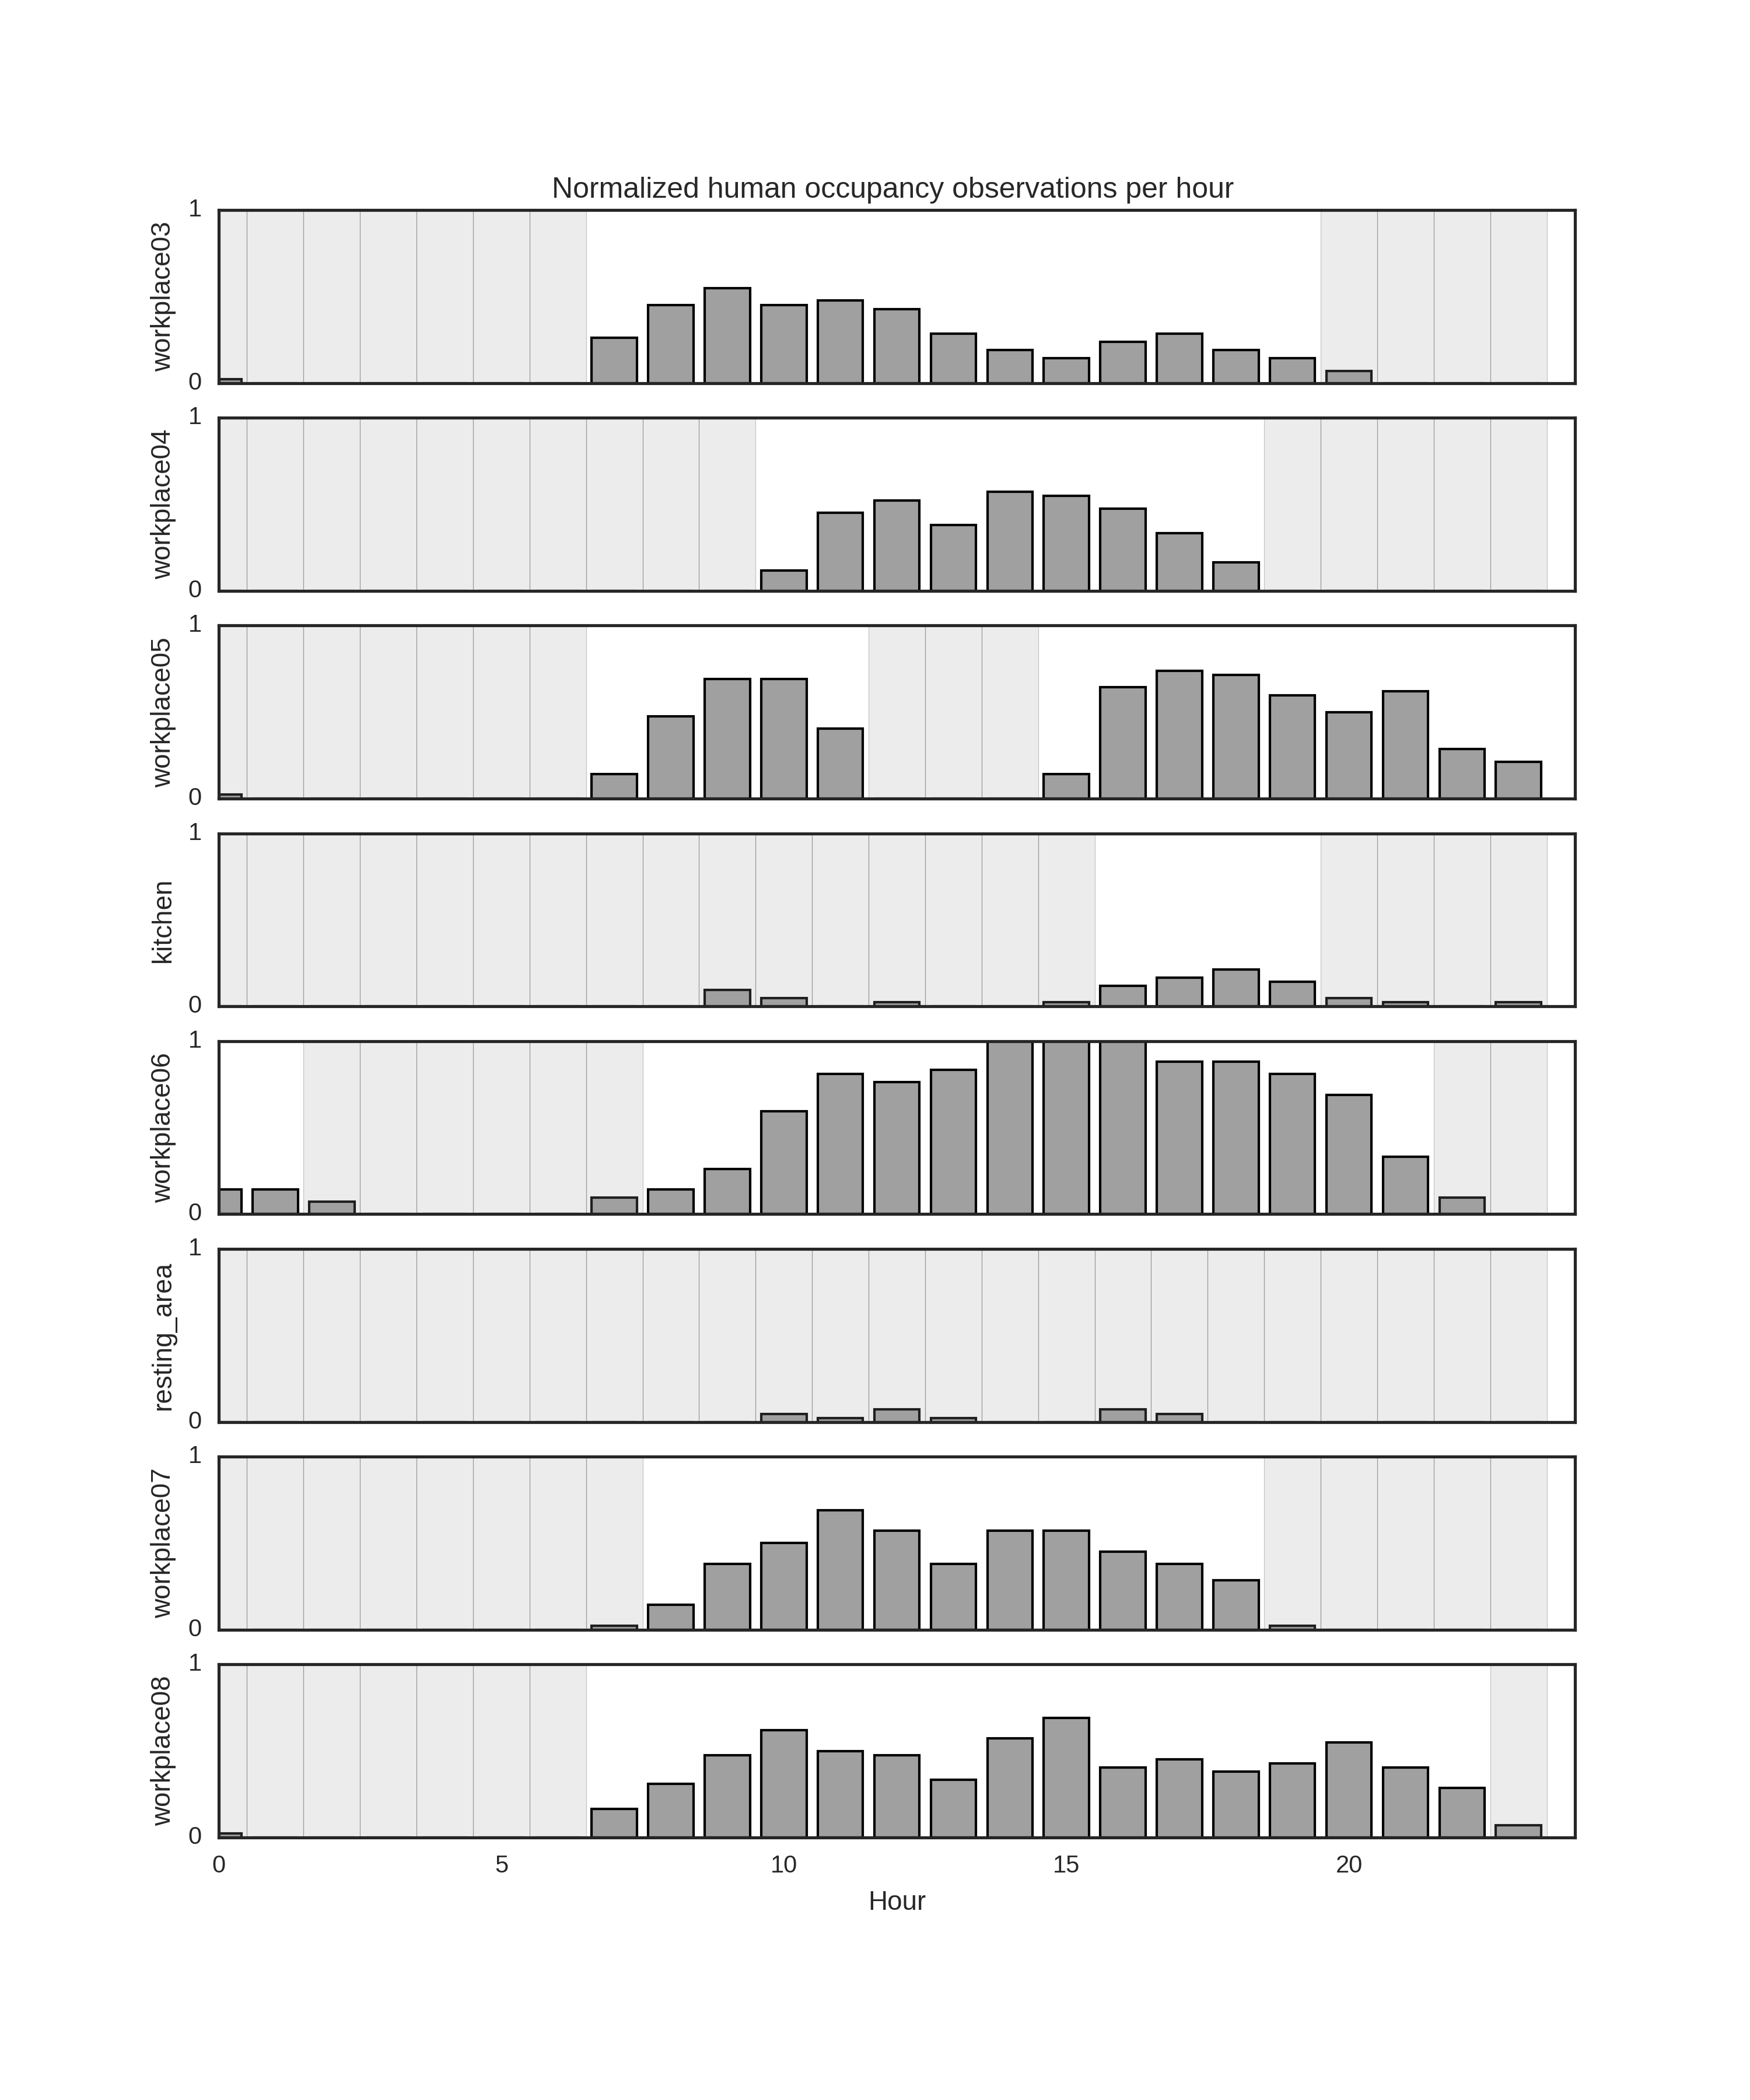
\includegraphics[width=\textwidth]{images/occupancy_hist_withresults.png}
\caption[Brayford Dataset ]{Brayford Dataset: Normalized human occupancy per hour per room. The shaded regions are the learned cleaning time period for each room.}
\label{fig:brayford_visualization}
\end{figure}

\FloatBarrier



The dataset is divided into training set and testing set. The training set consist of 2 weeks of observations where the robot visits the eight predefined locations of the office at a regular interval of 10 minutes. The test set consists of another week of observation. Figure~\ref{fig:brayford_visualization} is the bar plot of the observations made by the robot. The x axis is the time of the day, the columns are the different rooms of the office. We can see different patterns in different rooms like the resting area is least occupied thought out the day or workspace05 has a mid day break.
The training dataset was used to learn the parameters of the model while the testing dataset was used to predict and validate the learned models.
The accuracy results of the 8 rooms is plotted in Figure~\ref{fig:brayford_evaluation}. 

The model predicts with above \textbf{80\%} accuracy for 3 rooms kitchen, resting area and workplace04. While accuracy of predictions for three rooms are in the range of 60\% to 80\%.

\begin{figure}[htp]
\centering
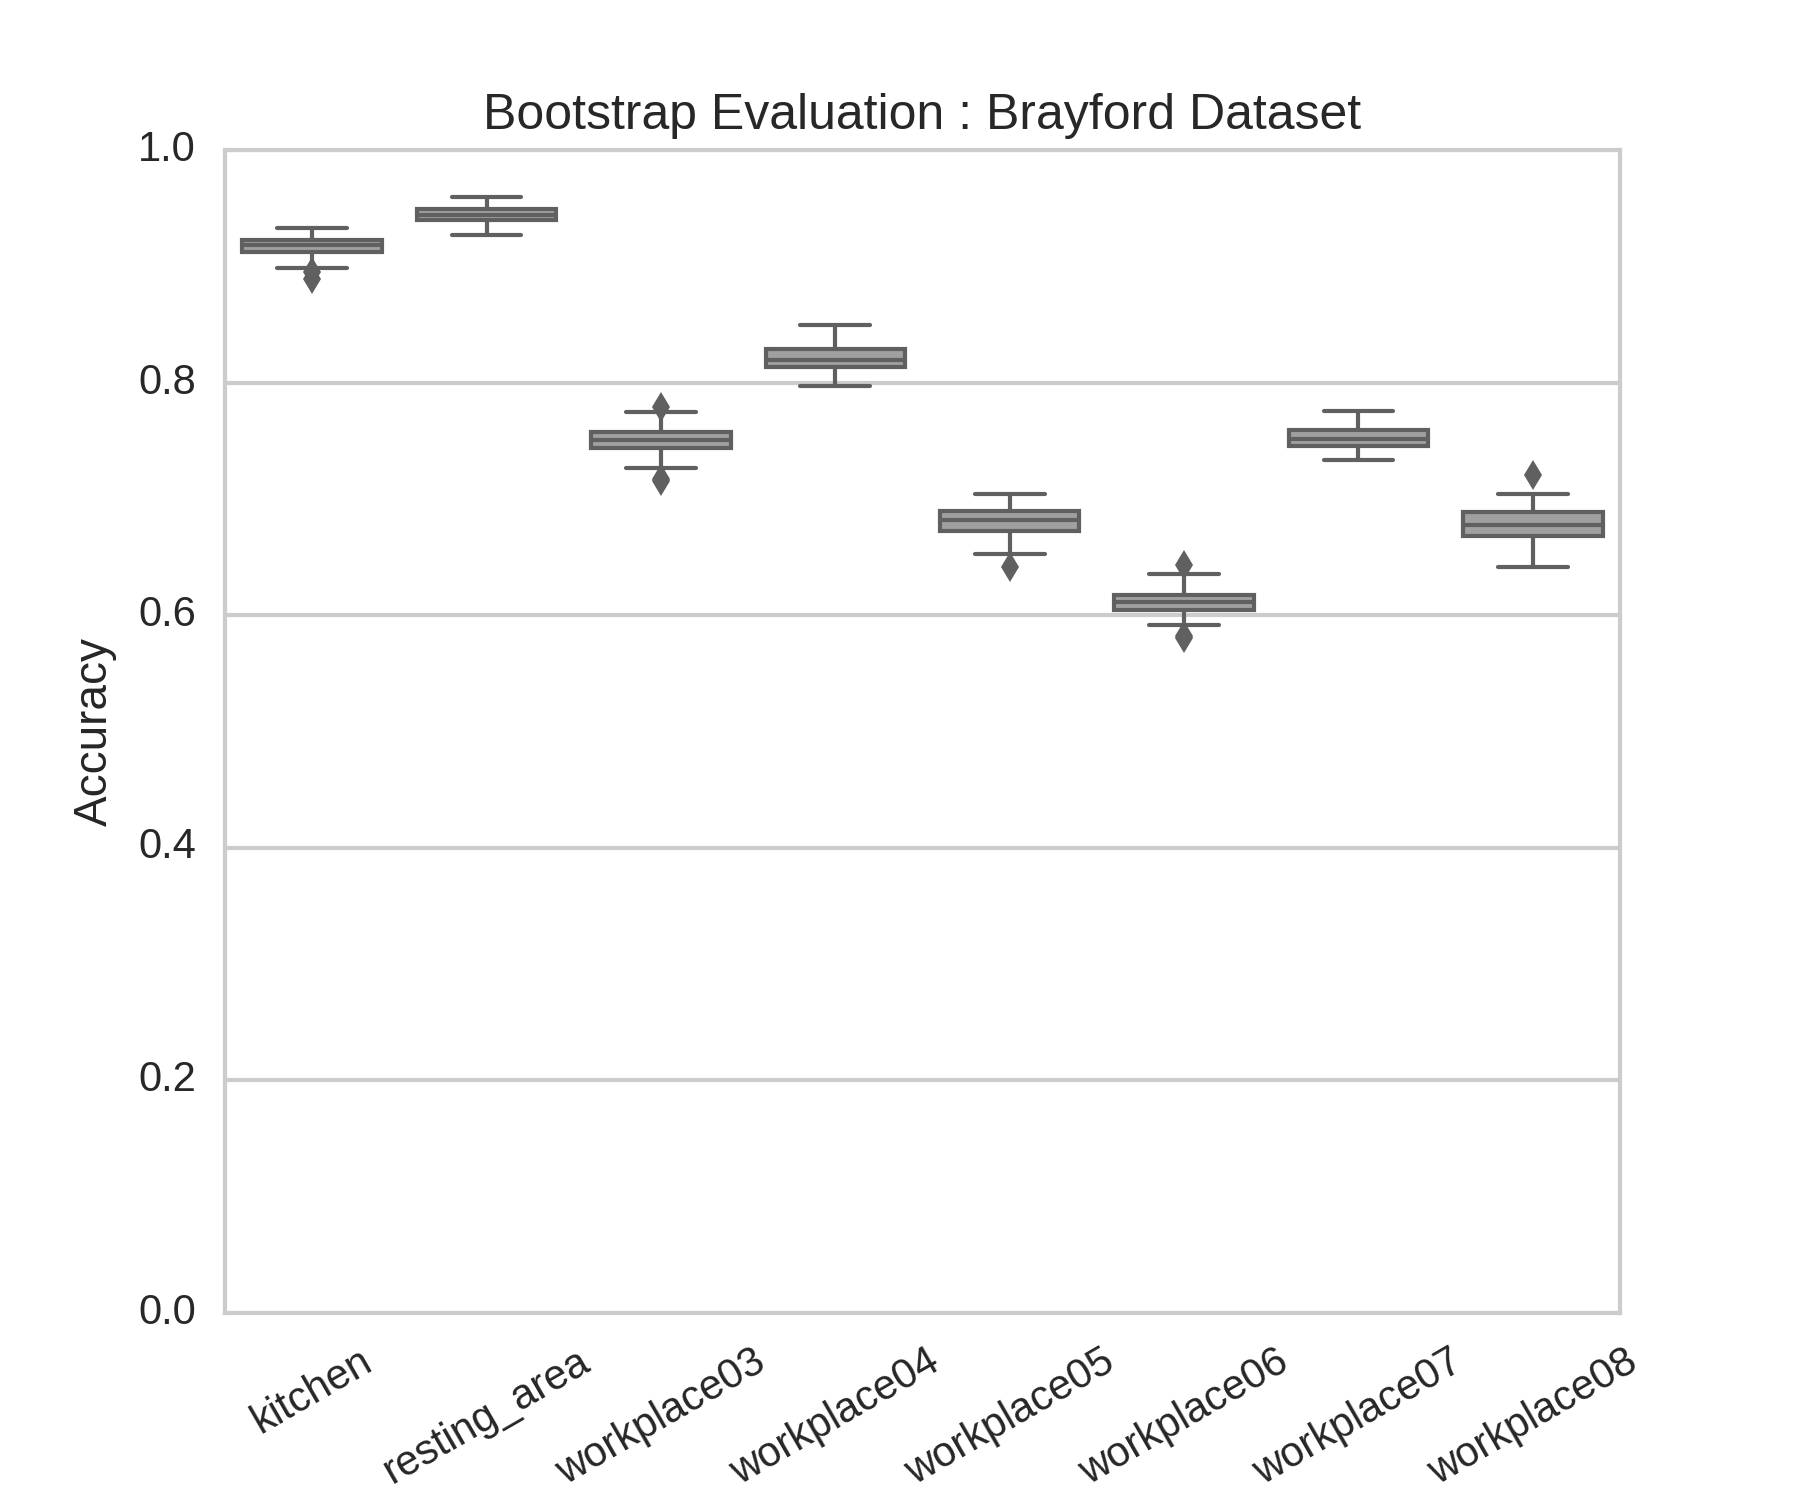
\includegraphics[width=0.7\textwidth]{images/Brayford_dataset_results_evaluation.png}
\caption[Brayford Dataset Evaluation]{Brayford dataset evaluation: Accuracy of the model for different rooms in the office}
\label{fig:brayford_evaluation}
\end{figure}



Based on the learned occupancy parameter for each room, the robot can now determine which are the periods of low occupancy and select these time periods for doing its cleaning task. We selected a threshold of $\theta_i < 0.2$ for low occupancy period. The shaded region in Figure~\ref{fig:brayford_visualization} are the learned low occupancy time periods in which the robot can perform cleaning task.
\FloatBarrier

\section{Discussions}

In this chapter, we presented a probabilistic model for learning the occupancy of each room in a environment. The robot continuously records in its robot memory when and where it saw the users. Based on the data collected, the robot gains knowledge about the occupancy of each room during different times of the day.

We have used the identical model as discussed in chapter ~\ref{chapter: object} for learning the occupancy parameter. This demonstrates flexibility of the probabilistic programming in which we can reuse the models in new problems.
From the experiments conducted on real world datasets collected by mobile robots in an open office we can conclude that the model is able to learn accurately the occupancy at different times of the day. One of the reasons for high accuracy is that the observations were made at regular fixed intervals, thus the model had enough evidence in each time-zone for learning also as there was an observable pattern to learn.